% !TEX encoding = UTF-8 Unicode
% !TEX TS-program = xelatex
\documentclass{article}
	\usepackage{tikz}
	\usepackage{fontspec}
		\setmainfont{PMingLiU}
\begin{document}
	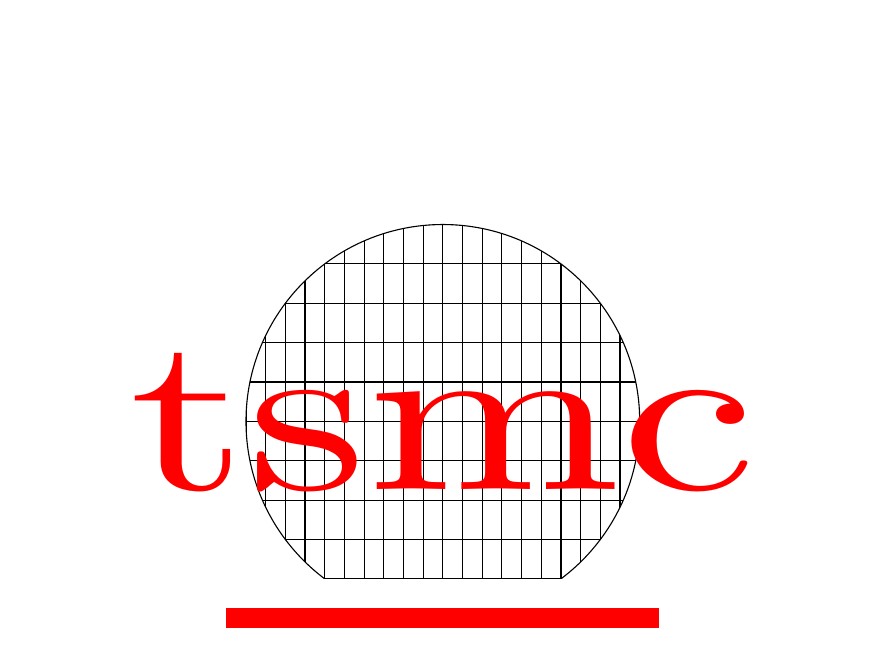
\begin{tikzpicture}[scale = 0.25]
		\begin{scope} % Wafer
			\draw (-6, -8) -- (6, -8) ;
			\clip (-20, -8) rectangle (20, 20) ;
			\draw circle [radius = 10] ;
			\clip circle [radius = 10] ;
			\foreach \x in {-10, ..., 10}{
				\draw (\x, -20) -- (\x, 20) ;
			}
			\foreach \y in {-5, ..., 5}{
				\draw (-20, \y*2) -- (20, \y*2) ;
			}
		\end{scope}
		\draw [red, line width = 2.5mm] (-11, -10) -- (11, -10) ;
		\node [red] at (0, 0) [xscale = 11, yscale = 8] {tsmc} ;
	\end{tikzpicture}
\end{document}